\section{Safety-Domain Validation Protocol and Complete Cases}
\label{app:safety_validation}
\noindent\textbf{Correspondence: Section~\ref{sec:evaluation}.}
This appendix records the qualitative checks of the configuration
conditions and certified comparison. The original reference/actual
protocol and the uniform-interval annex were frozen separately before
their respective runs. Gain selection was not part of either batch.
The examples were chosen using known theory and earlier traces to
test mechanisms, not to estimate an independent population advantage.

\subsection{Reference configurations and verification}
All cases use $C=2048$, the bidirectional triangle,
$H=h=30000000/29999$, $k_p=2\times10^{-6}$,
$k_i=5\times10^{-11}$ and
$(K_e,K_{\Delta e},K_u)=(0.1,29999/7500,-768/18749375)$.
Memory is zero, phases are equal and $\omega_{\rm ref}=29999/30000$.
The prescribed uncontrolled offsets are
$s(7,-5,-2)^\top/30000$. Link and execution delays are zero only in
the reference. The continuous plant is exactly integrated between
held corrections; there is no Euler approximation or replacement by
a discrete firing-count plant. The reference executes the original
25-rule surface and the implemented integrate-first PI.

Twelve direct runs at $s=1$ use $z=16,20,24,2024,2028,2032$.
Initial occupancy, target and compatible marking all equal $z$.
There are two cases in which both unprotected references cross,
two in which both are safe, and two with strict Fuzzy safety but
PI crossing, accounting for the upper/lower mirror.
The point comparison gives Fuzzy's all-time interval
$(z-17.315,z+17.315)$, whereas PI attains the exact enclosed
excursion of about 23.403701 frames. The shadow virtual continuation
after a first crossing is retained for diagnostics and is not a
physically admissible buffer trace.

The mismatch-source grid is
$s=0.25,\allowbreak0.5,\allowbreak0.75,\allowbreak0.85,\allowbreak0.86,\allowbreak1,\allowbreak1.125,\allowbreak1.25,\allowbreak1.5,\allowbreak2$.
Six sources at $s=0.5,1,2$ are reused only after configuration,
source and raw hashes are verified; the other 14 are new.
Their finite-horizon extrema determine sampled occupancy intervals
by the proved translation identity. No extra plant run is charged
for this derived map. Successful columns do not imply that the
unsampled region is certified. The joint Lyapunov certificate is
evaluated separately, including input-domain, limiter and positive-
frequency conditions. The earlier midpoint grid certifies PI through
$s=16$ and Fuzzy through $s=2$ under their respective coarse tests;
this is not a true safe-set ordering.

Four further runs test $(6,-6,0)/30000$ and
$(8,-4,-4)/30000$ at $z=1024$. Alongside the prescribed direction,
their pairwise initial spreads are all 400 ppm and their means
coincide. However, $Q=\delta\omega^\top L\delta\omega$ takes values
$(216,234,288)/30000^2$. The exact energy identity is checked;
PI's peaks coincide here because of the triangle's repeated
disagreement eigenvalue, while Fuzzy's peaks differ. Thus the energy
condition is sufficient and distribution-aware, without predicting
a strict ordering of measured peaks.

\begin{figure*}[t]
 \centering
 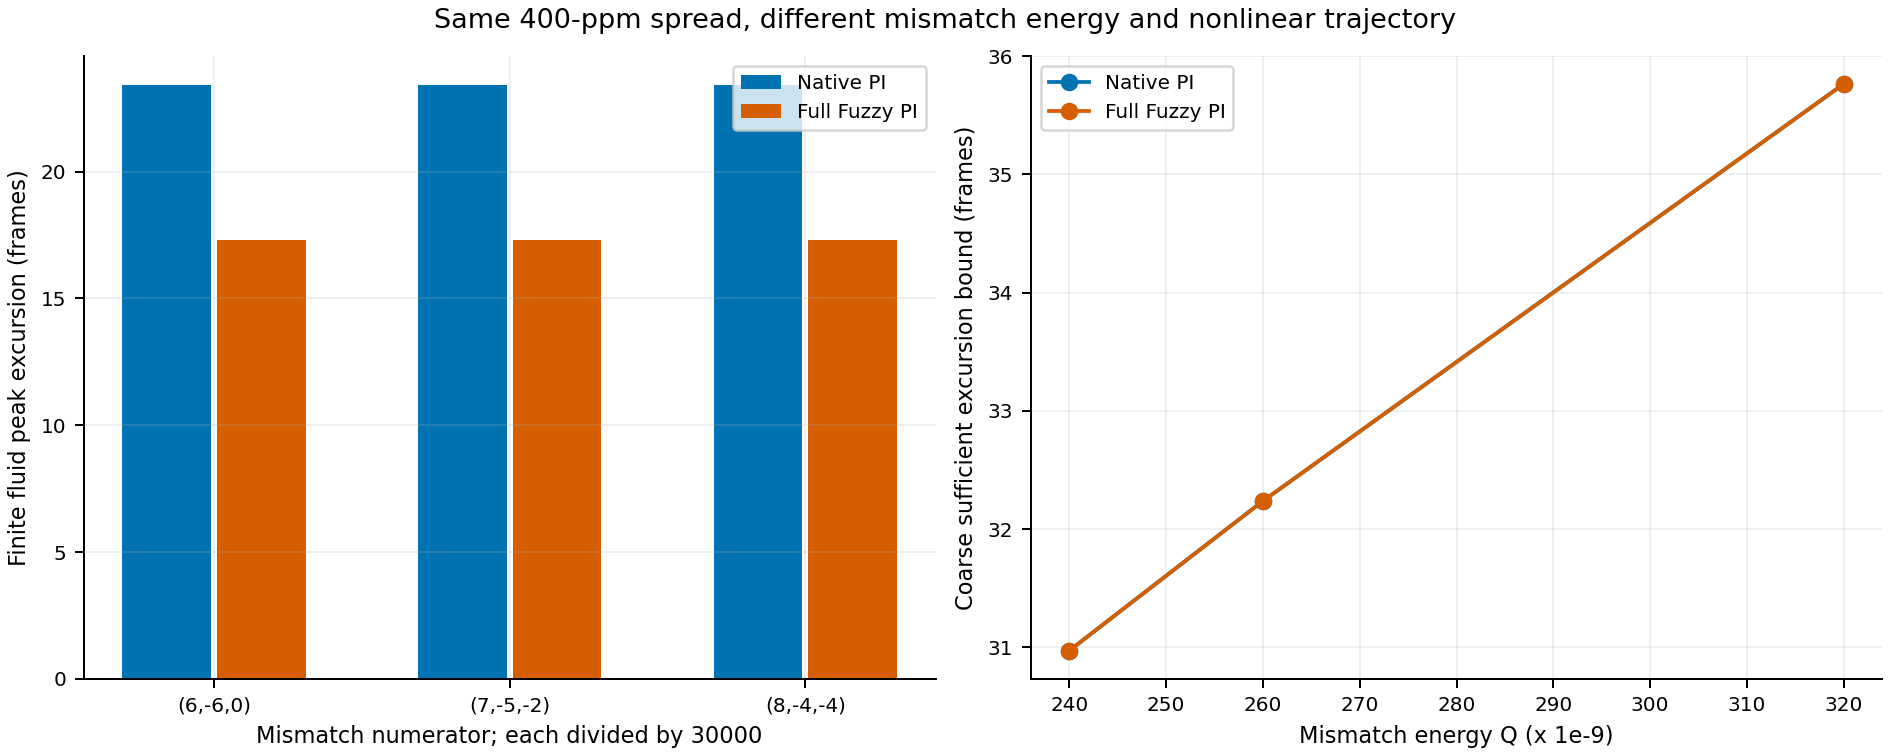
\includegraphics[width=0.94\textwidth]{images/safety_validation_20261105/direction_energy.png}
 \caption{Three equal-spread initializations with different mismatch
 energy. The energy identity is exact; a larger certificate radius
 does not imply a larger exact trajectory peak.}
 \Description{Mismatch energies and controller excursions for three 400-ppm directions.}
 \label{fig:safety_direction_energy}
\end{figure*}

The separately frozen annex adds four runs at $s=0.999,1.001$,
$z=20$. It independently recomputes every outward-arithmetic
cell of the uniform proof. Fuzzy's endpoint minima are approximately
2.703366 and 2.668520; PI's are $-3.380298$ and $-3.427105$.
The endpoint runs check implementation consistency. The 20-cell
coverage and infinite-tail argument, not endpoint interpolation,
establish the all-time statement over the entire interval.

\begin{figure*}[t]
 \centering
 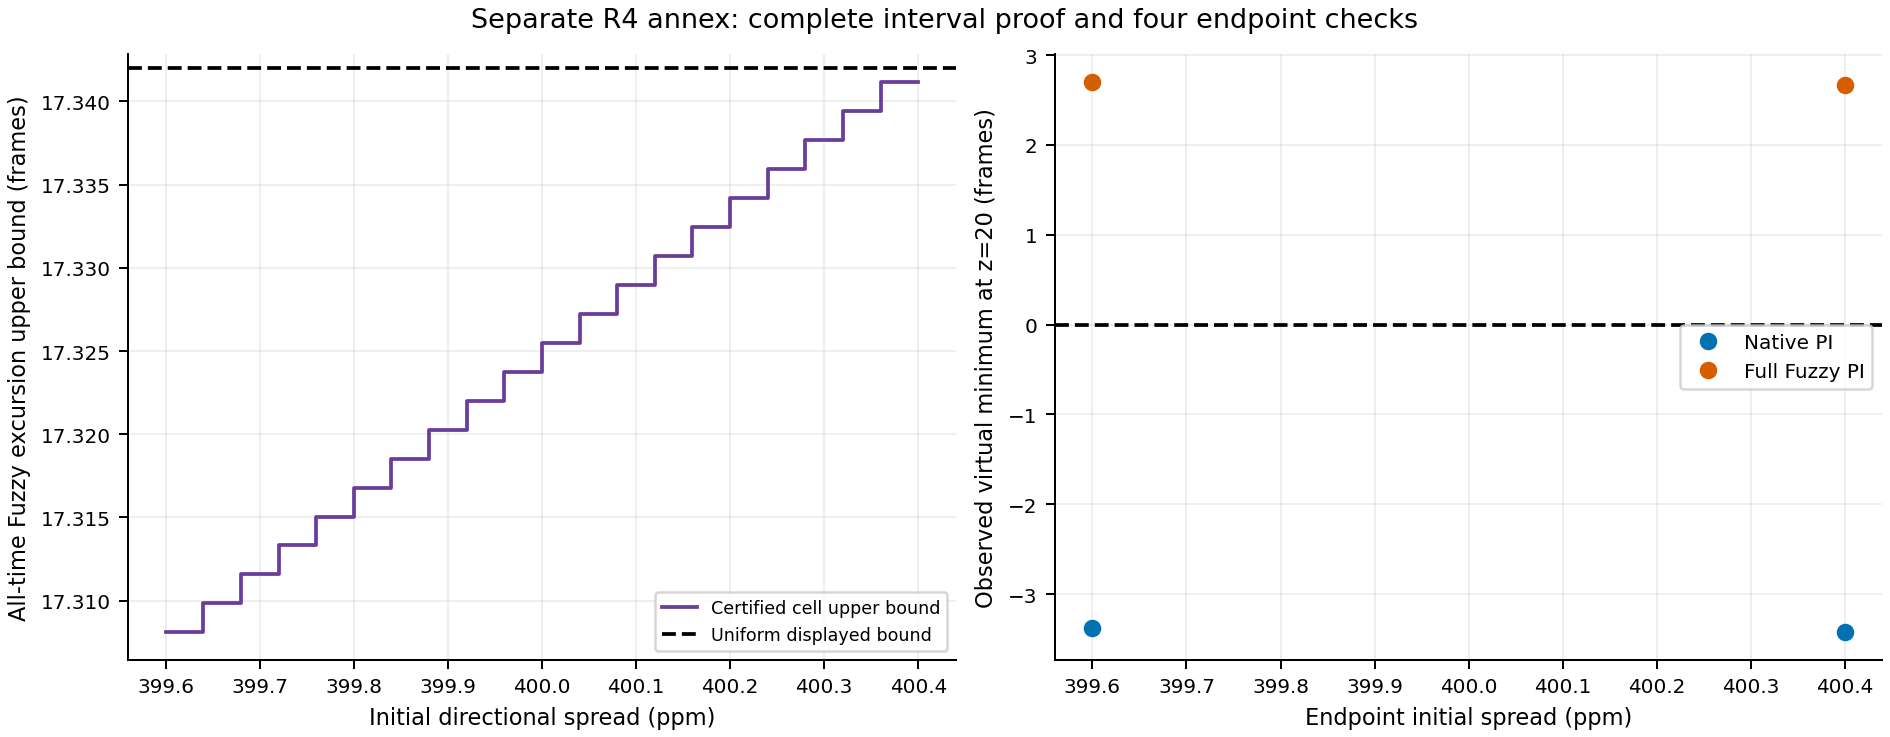
\includegraphics[width=0.94\textwidth]{images/safety_validation_20261105/uniform_annex_R4.png}
 \caption{Complete parameter-cell proof and direct endpoint checks.
 All 20 cells cover 399.6--400.4 ppm at the fixed mismatch direction.
 The maximum Fuzzy all-time bound is below 17.342; PI's minimum
 attained peak exceeds 23.3802976 throughout the interval.}
 \Description{Uniform interval bounds and four reference endpoint validations.}
 \label{fig:safety_uniform_interval}
\end{figure*}

All reference runs use bootstrap plus 2000 subsequent intervals.
Maximum translation residual is $6.83\times10^{-13}$ frame and
maximum phase residual $2.78\times10^{-12}$. The original comparison
tolerances are unchanged. Interpolation and rule replay are checked
separately from the exact proof certificate. The record contains
34 new reference trajectories, six cached sources and separate
proof/postprocessing evidence.

\subsection{All delayed Callisto cases}
The actual runs restore physical link latency 20, local polling
1000, execution delay 10 and integer events over $T=2001H$.
They fix $s=4$, initial phase 0.1, all capacities and gains above,
and use the original negative-time source history. For each $z$,
PI's target is $z$, Fuzzy's percentage setpoint is $100z/2048$,
and the marking is initial occupancy plus initial in-flight frames.
Each paired history and marking is identical. Guards are enabled
with reserve zero; observer, supervisory switching and anti-windup
are disabled. Requested/resolved settings are checked before
results are used.

\begin{table*}[t]
 \caption{All actual qualitative validation cases. Occupancy extrema
 include every integer event. Blocked time sums disabled-data-phase
 duration across nodes, rather than measuring elapsed network downtime.}
 \label{tab:safety_actual_all}
 \centering
 \begin{tabular}{@{}rllrrl@{}}\toprule
 $z$ & Controller & Buffer range / frames & Off episodes & Blocked node-ticks & First guard cause\\\midrule
 104 & PI & 10--198 & 0 & 0 & none\\
 104 & Fuzzy & 32--176 & 0 & 0 & none\\
 83 & PI & 0--166 & 5 & 61.0114 & empty input\\
 83 & Fuzzy & 11--155 & 0 & 0 & none\\
 64 & PI & 0--128 & 26 & 131.0456 & empty input\\
 64 & Fuzzy & 0--128 & 6 & 47.0093 & empty input\\
 1944 & PI & 1880--2008 & 26 & 131.0456 & delayed outgoing credit\\
 1944 & Fuzzy & 1880--2008 & 6 & 47.0093 & delayed outgoing credit\\
 1965 & PI & 1922--2008 & 51 & 222.1022 & delayed outgoing credit\\
 1965 & Fuzzy & 1922--2008 & 3 & 84.0205 & delayed outgoing credit\\
 1984 & PI & 1960--2008 & 5837 & 587.8914 & delayed outgoing credit\\
 1984 & Fuzzy & 1960--2008 & 1198 & 188.3495 & delayed outgoing credit\\\bottomrule
 \end{tabular}
\end{table*}

At $z=83$ PI's first input-empty guard occurs at
$t\simeq71844.671848$ ticks; five episodes sum to about 61.0114
blocked node-ticks. Fuzzy remains unstalled. The physical clock
continues to advance when data phase pauses, so physical-phase and
data-phase progress must be recorded separately.

\begin{figure*}[t]
 \centering
 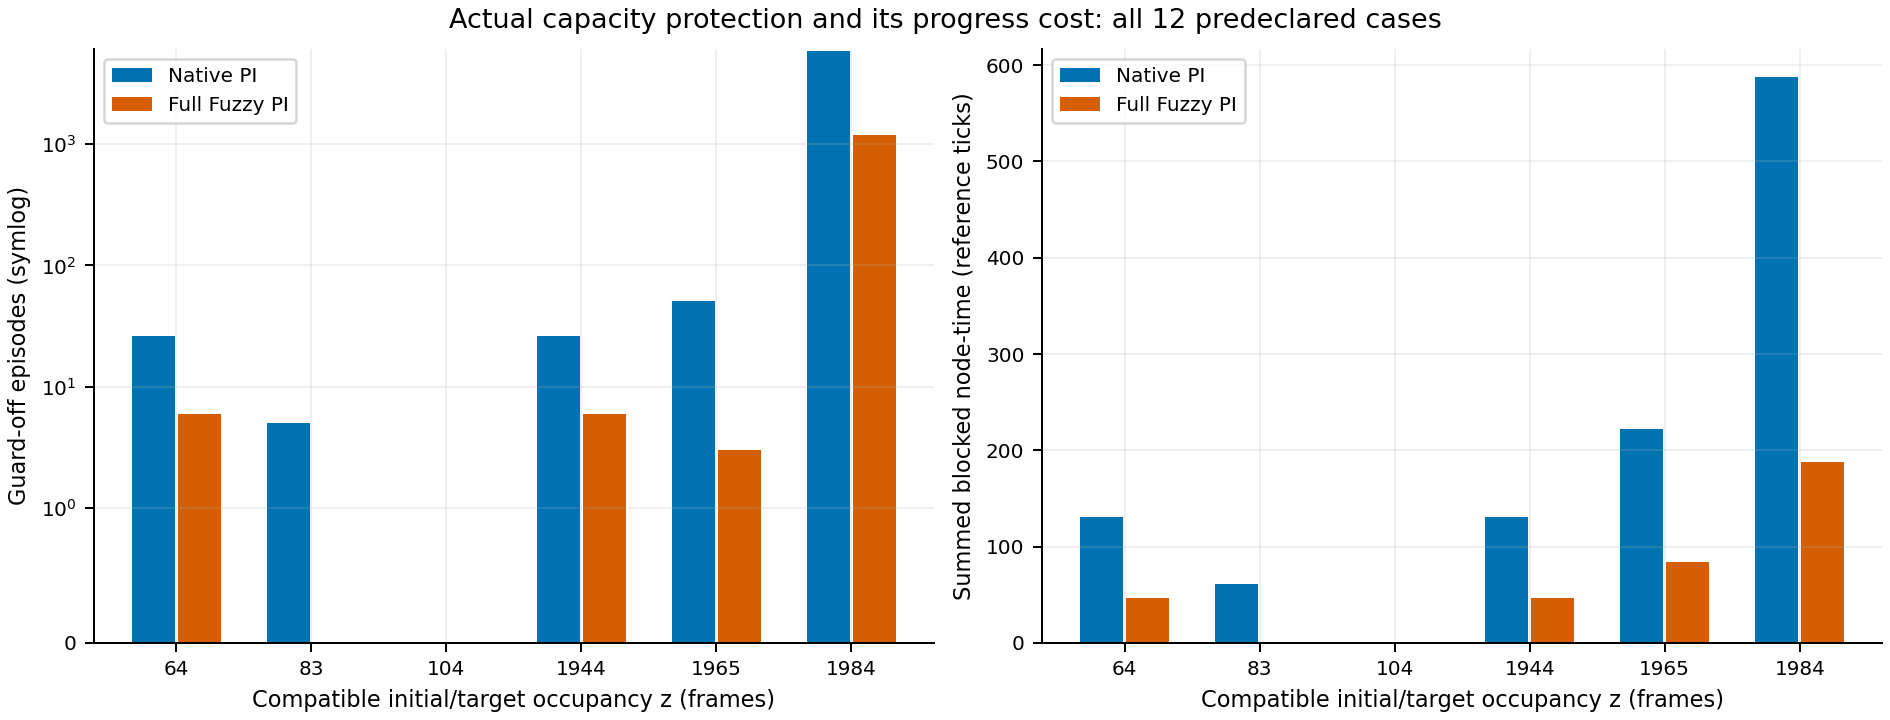
\includegraphics[width=0.94\textwidth]{images/safety_validation_20261105/actual_guard_comparison.png}
 \caption{Guard-off episodes and summed blocked node-time for every
 predeclared actual case. Three cases remain unstalled. Nine retain
 capacity with guard intervention; counts alone are not throughput.}
 \Description{Both normal and guarded outcomes, without omitting high-target cases.}
 \label{fig:safety_guard_comparison}
\end{figure*}

Upper-target cases do not reproduce the receiving-buffer mirror
of the zero-delay reference. In this runtime, used outgoing credit
is the UGN offset plus source sends minus causally delayed reverse
pops. Its initial value is $z+40$ although initial receiving occupancy
is $z$: the accounting includes forward in-flight data and delayed
reverse consumption knowledge. Full credit replay verifies its
capacity constraint. All upper-target cases guard while the maximum
physical receiving occupancy remains 2008. The first credit guards
at $z=1944$ occur at approximately 47886.861480 ticks (PI) and
57745.333282 ticks (Fuzzy), matching the corresponding $z=64$
lower-target cases. This explains the discrepancy without changing
gains. The observed 40-frame difference is specific to the declared
constant latency, history and protocol; it is not a general delay
margin or an all-time theorem for Callisto.

\begin{figure*}[t]
 \centering
 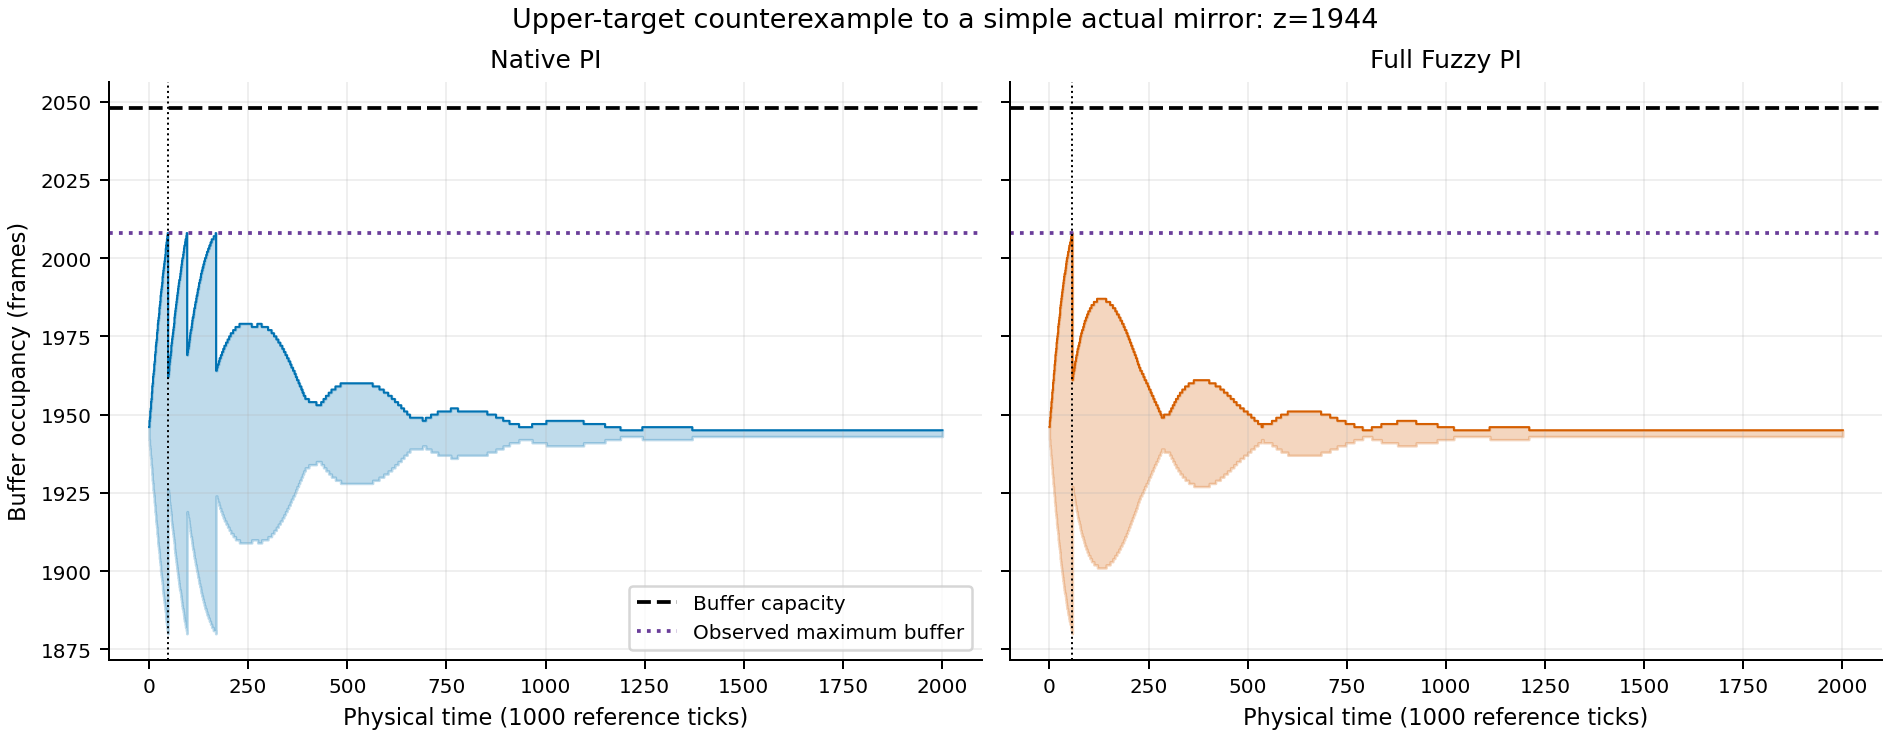
\includegraphics[width=0.94\textwidth]{images/safety_validation_20261105/actual_upper_credit.png}
 \caption{Actual upper-target credit constraint at $z=1944$.
 Credit readiness can stop sending before receiving occupancy reaches
 capacity. Forward in-flight frames and delayed reverse-pop knowledge
 prevent an occupancy-only upper/lower mirror argument.}
 \Description{Receiving buffers and delayed outgoing-credit guards in the upper-target case.}
 \label{fig:safety_upper_credit}
\end{figure*}

Every actual run has positive physical frequency (minimum 0.9993)
and no saturated correction. Complete integer arrival/pop replay
has zero occupancy mismatches; independent PI/25-rule command
reconstruction has maximum residual $1.09\times10^{-19}$.
Pre-first-guard measurements, command times and corrections agree
with the high-reserve source trajectory. Subsequent evolution is
from independent actual runs, not shifted old curves. All 12 runs
remain within inclusive physical capacity; the nine guarded cases
do not establish controller-only strict interior safety. At $z=1965$,
Fuzzy has fewer guard episodes but lower final data progress than
PI, so neither episode count nor blocked duration alone demonstrates
a throughput improvement.

\subsection{Claim--evidence separation}
Exact matrix/interval calculations certify the reference inner
domain, strict target-interval benefit and uniform narrow directional
interval. Reference simulation checks the original rules and model
identities. Delayed actual runs check whether the margin mechanism
persists, and expose an additional credit condition. They do not
certify arbitrary topology, delay, initial error at a fixed target,
globally optimal PI comparison, or application-payload logical
synchrony. Earlier random, burst and independently tuned comparisons
remain separate supplementary evidence in Appendix~\ref{app:evaluation}.
